% Ubah judul dan label berikut sesuai dengan yang diinginkan.
\section{Metodologi}
\label{sec:metodologi}

% Ubah paragraf-paragraf pada bagian ini sesuai dengan yang diinginkan.

\section{Metode yang digunakan}

Berikut ini adalah metode yang digunakan

% Contoh input gambar dengan format *.jpg
\begin{figure}  \centering
  % Nama dari file gambar yang diinputkan
  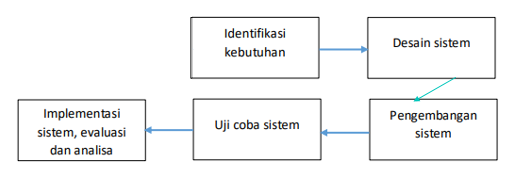
\includegraphics[scale=0.45]{gambar/Screenshot 2023-06-10 193529.png}
  % Keterangan gambar yang diinputkan
  \caption{Metodologi Penelitian}
  % Label referensi dari gambar yang diinputkan
  \label{fig:Metodologi}
\end{figure}

% Contoh penggunaan referensi dari gambar yang diinputkan
Gambar \ref{fig:Metodologi} menjelaskan tentang metodologi penelitian.

\section{Bahan dan peralatan yang digunakan}
Dalam penelitian ini, digunakan bahan dan peralatan yang dibutuhkan.
\subsection {Perangkat keras (hardware)}
Perangkat keras yang digunakan adalah sebagai berikut.
\begin{itemize}
 \item Laptop
 \item Mikrokontroler ESP32
 \item \emph{Webcam}
\end{itemize}

\subsection {Perangkat lunak (software)}
Perangkat lunak yang digunakan adalah sebagai berikut.
\begin{itemize}
 \item Arduino IDE
 \item Visual Studio Code
 \item GitHub
\end{itemize}


% Contoh input beberapa gambar pada halaman.
\begin{figure*}
  \centering
  \subfloat[Hasil A]{\includegraphics[width=.4\textwidth]{example-image-a}
    \label{fig:hasila}}
  \hfil
  \subfloat[Hasil B]{\includegraphics[width=.4\textwidth]{example-image-b}
    \label{fig:hasilb}}
  \caption{Contoh input beberapa gambar.}
  \label{fig:hasil}
\end{figure*}

\lipsum[16-18]

% Contoh input potongan kode dari file.
\lstinputlisting[
  language=Python,
  caption={Program perhitungan bilangan prima.},
  label={lst:bilanganprima}
]{program/bilangan-prima.py}

\lipsum[19-20]
